\chapter{Results}
\label{chap:results}
\begin{figure}[h!]
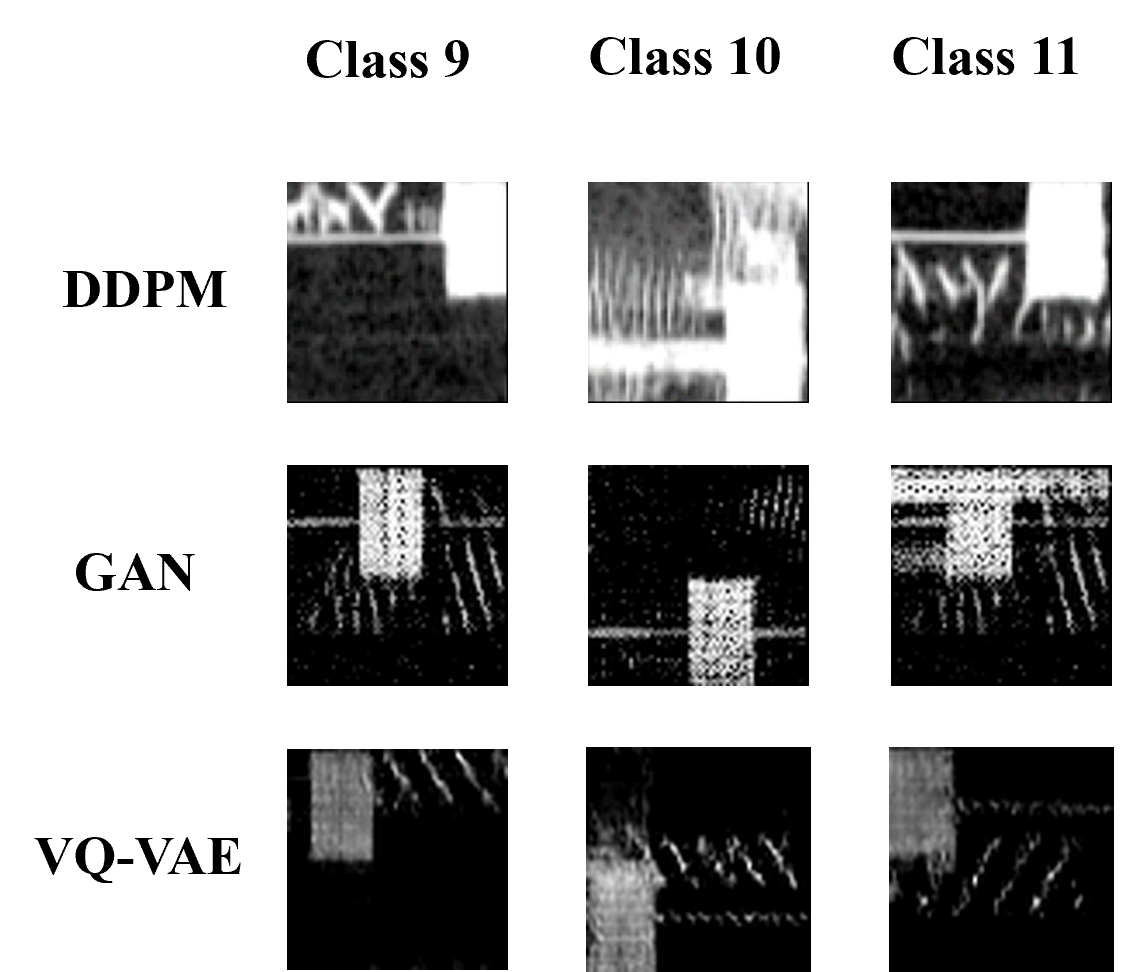
\includegraphics[width=10cm]{figures/Picture7.png}
\centering
\caption{A side-by-side comparison of some of the collision scenarios generated by the \gls{ddpm}, the \gls{gan}, and the \gls{vq-vae} }
\centering
\end{figure}

Classes depicted in Figure 3.1: class 9, class 10, and class 11 are all collision scenarios (Refer to Figure 2.1), which were generated by the \gls{ddpm}, the \gls{gan}, and the \gls{vq-vae}. 

\begin{figure*}[ht]
    \centering
    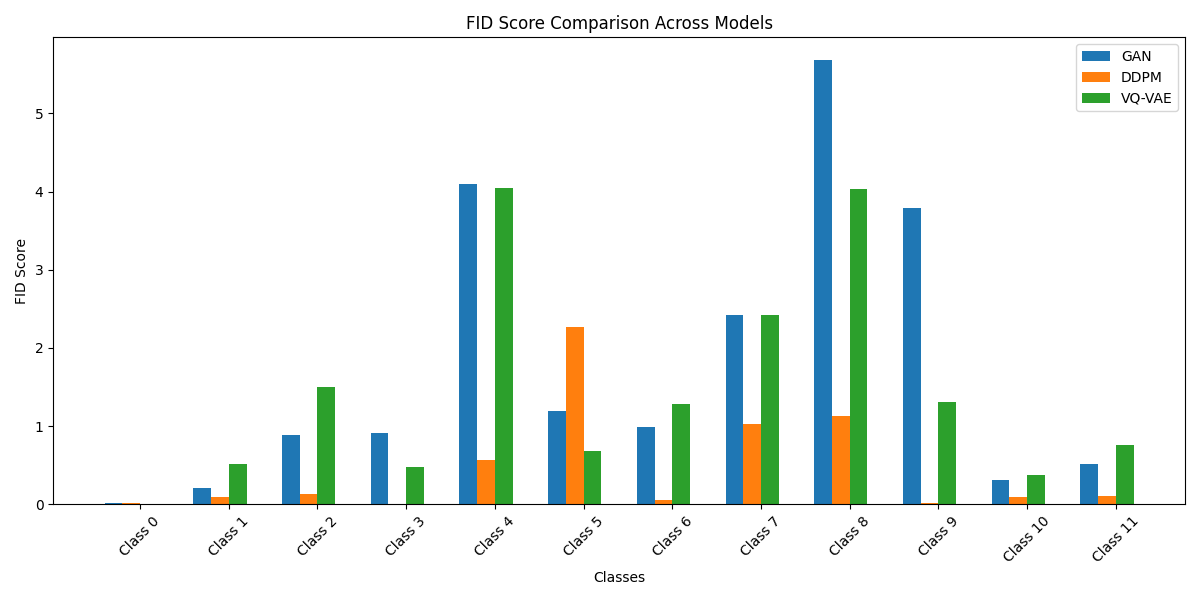
\includegraphics[width=\textwidth]{figures/Figure_12.png} 
    \caption{\gls{fid} Score Comparison Across Models for Different Classes.}
    \label{fig:fid_scores}
\end{figure*}
Figure 3.2 illustrates the change in \gls{fid} score across the classes for the 3 models.  The \gls{gan}, \gls{ddpm}, and \gls{vq-vae} models achieved average \gls{fid} scores of 1.944, 0.504, and 1.580, respectively. We used a ResNet18 model with the final classification layer replaced to extract features instead of using a pre-trained InceptionV3 network due to the specific nature of our dataset.

Since our dataset lacks the complex textures, patterns, and color information typically found in natural image datasets, the differences between real and generated spectrograms are smaller in the feature space. As a result, the \gls{fid} scores we obtained are smaller than usual for all three models.

Class 0 consistently shows near-zero \gls{fid} scores across all three models due to its purely noise-like nature. As observed in the graph, the classes representing collision scenarios—Class 9, Class 10, and Class 11—exhibit significantly lower \gls{fid} scores for images generated by the \gls{ddpm}. This suggests that the spectrogram images with collision scenarios generated by the \gls{ddpm} are more natural and resemble the original dataset better than the other two models. The other two models also have relatively low \gls{fid} scores for Class 10 and Class 11.

Among the three models, the \gls{ddpm} also has the lowest average \gls{fid} score, suggesting that \gls{ddpm} is the most effective model overall for generating spectrograms that closely resemble the real dataset, as evidenced by its consistently low \gls{fid} scores across most classes.

The \gls{gan} model's high \gls{fid} scores across many classes suggest model collapse in its generated spectrograms for this dataset, to which \gls{gan}s are susceptible. Given that our main focus is on generating a diverse dataset to improve the accuracy of a visualized interference classification system, having a wide variety of data is essential.

\gls{vq-vae} model, on the other hand, shows varied performance, outperforming \gls{gan} in many cases (e.g., Classes 1, 2, 6, 9) but falling behind \gls{ddpm} in most.

\begin{figure}[h]
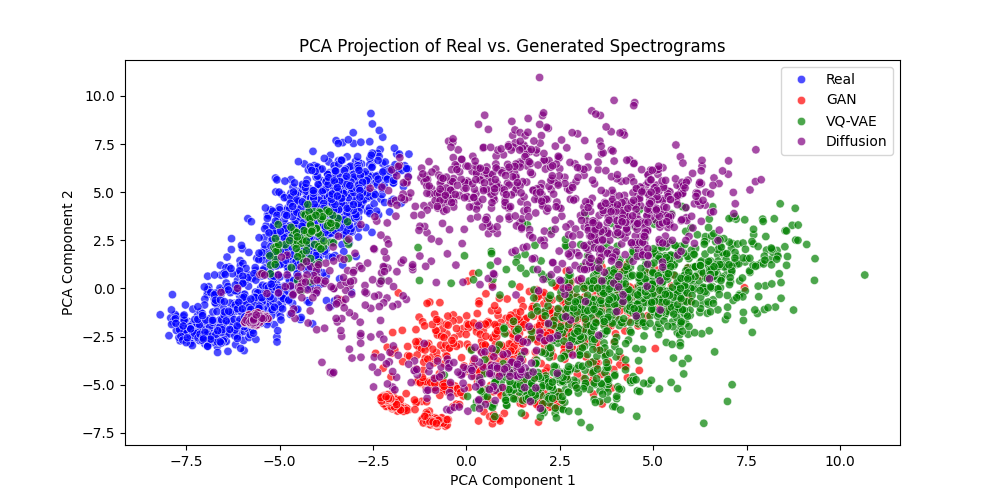
\includegraphics[width=\textwidth]{figures/PCA (1).png}
\centering
\caption{ \gls{pca} scores for the \gls{gan}, \gls{ddpm} and \gls{vq-vae}}
\centering
\end{figure}
The \gls{pca} projection in Figure 3.3 indicate that real and generated spectrograms form separate yet overlapping clusters, suggesting that generative models do not simply reproduce existing samples but introduce new variations. The spread of generated samples in the \gls{pca} projection indicates that the models create additional variations, potentially improving classifier generalization. The \gls{pca} analysis provides an independent validation of data distribution differences, confirming that generative models add meaningful diversity.

